\documentclass[12pt,a4paper]{article}
\usepackage{graphicx}
\usepackage{amsmath}
\usepackage{bm}
\usepackage{interval}
\begin{document}
\section*{Problem 11}    

\begin{figure}[hbp]
    \centering
    \begin{minipage}{0.48\linewidth}
        \centering
        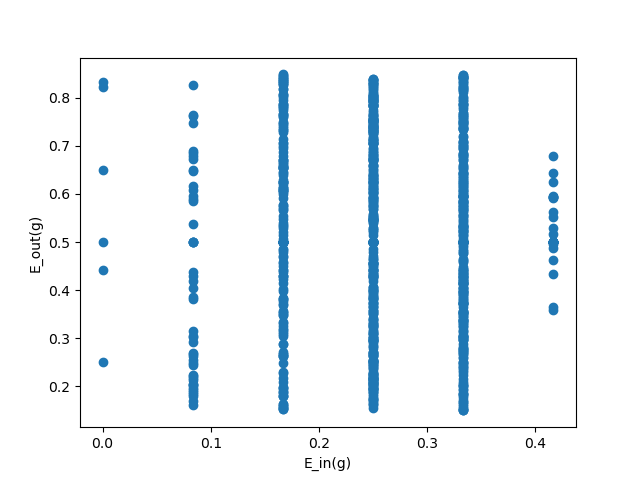
\includegraphics[width = \linewidth]{Hw2P11.png}
        \caption{scatter plot}
    \end{minipage}\hfil
    \begin{minipage}{0.48\linewidth}
        \centering
        
\includegraphics[width = \linewidth]{Hw2P11 median.png}
        \caption{median}
    \end{minipage}\hfil
    \centering
    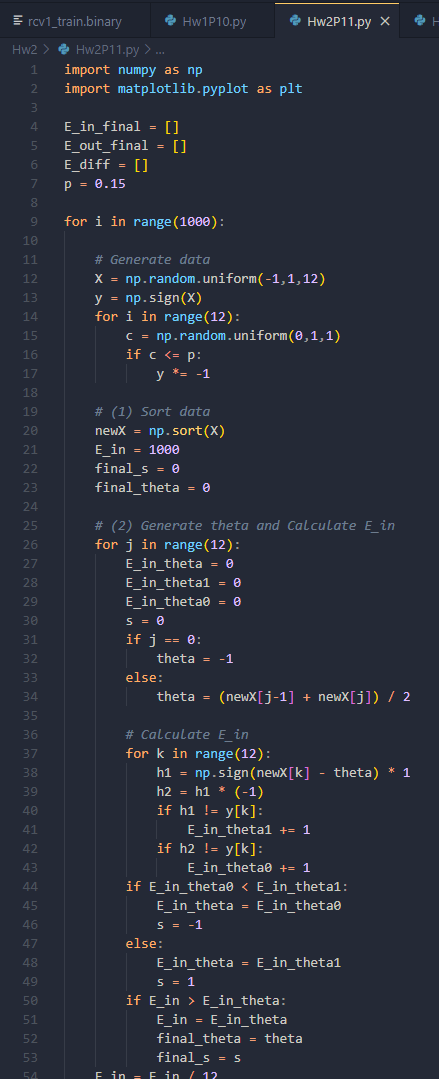
\includegraphics[height = 0.4\textheight]{Hw2P11 snapshot.png}
    \caption{snapshot}
\end{figure}

\newpage
\section*{Problem 12}    
For the P11, we choose $\theta, s$ to minimize $E_{in}$. And now, we choose $\theta, s$ uniformly.
From the median, we can easily observe that the $E_{out}-E_{in}$ is almost 0.
The conclusion is that if we choose $\theta, s$ to minimize $E_{in}$, we will have more $E_{out}-E_{in}$,
while if we choose $\theta, s$ uniformly, we can minimize $E_{out}-E_{in}$ but we will have more $E_{in}$.
\begin{figure}[hbp]
    \centering
    \begin{minipage}{0.48\linewidth}
        \centering
        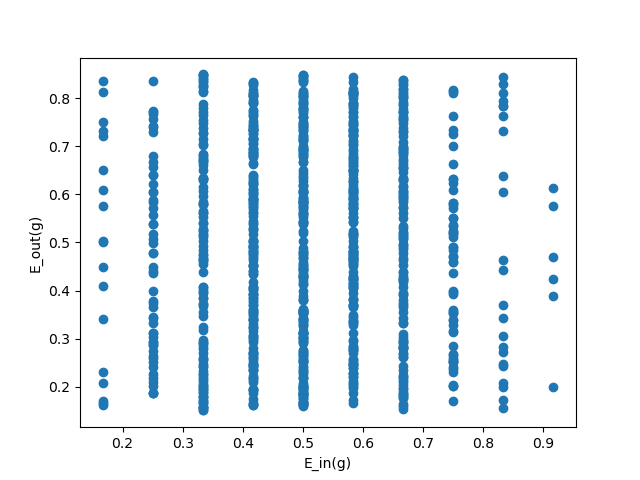
\includegraphics[width = \linewidth]{Hw2P12.png}
        \caption{scatter plot}
    \end{minipage}\hfil
    \begin{minipage}{0.48\linewidth}
        \centering
        
\includegraphics[width = \linewidth]{Hw2P12 median.png}
        \caption{median}
    \end{minipage}\hfil
\end{figure}
\end{document}
